\section{Geometry Variations}

\begin{figure} \label{fig:geo}
  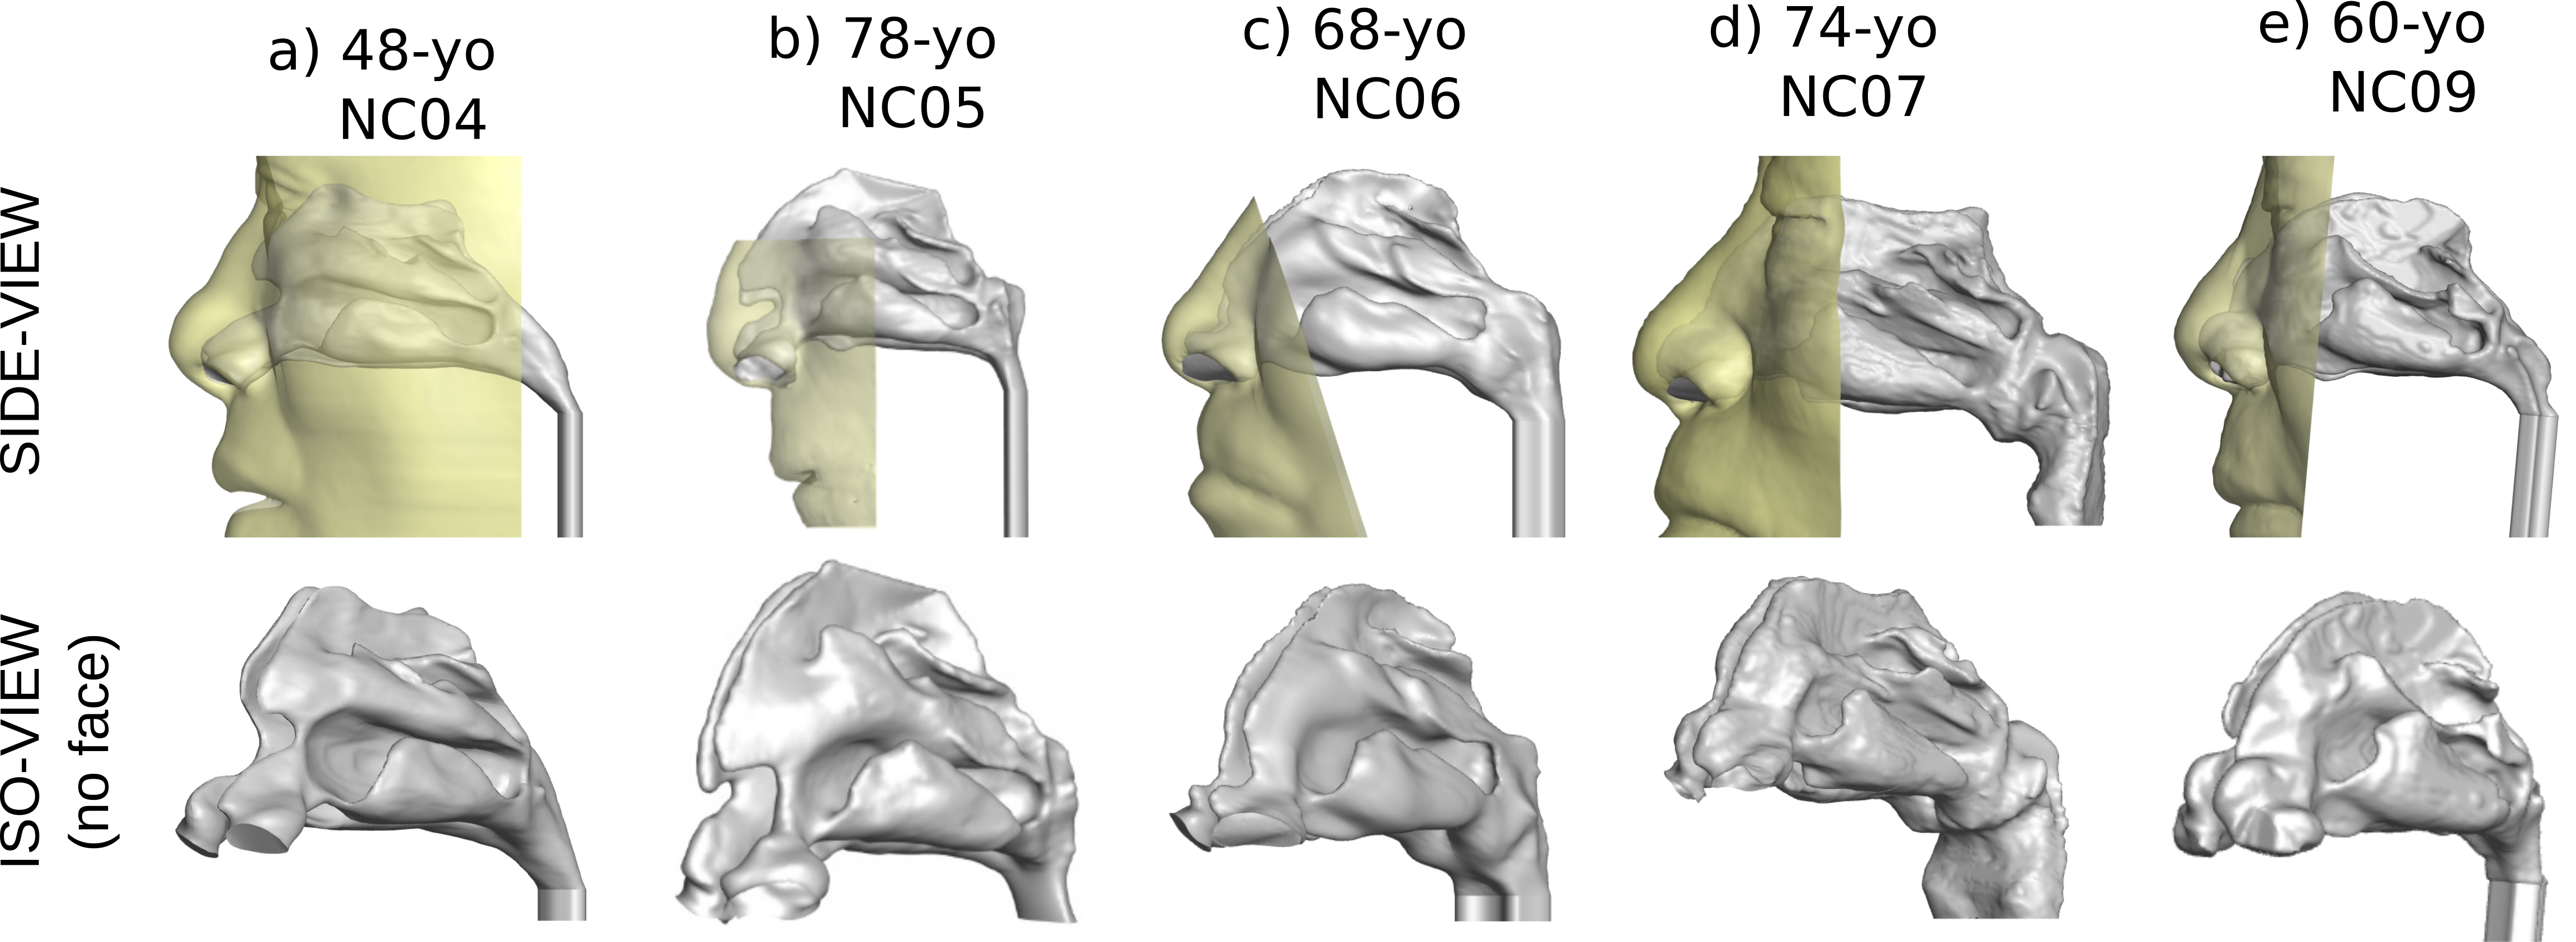
\includegraphics{geometries}
  \caption{geometries of the five cavities}
\end{figure}

\begin{figure} \label{fig:sil}
  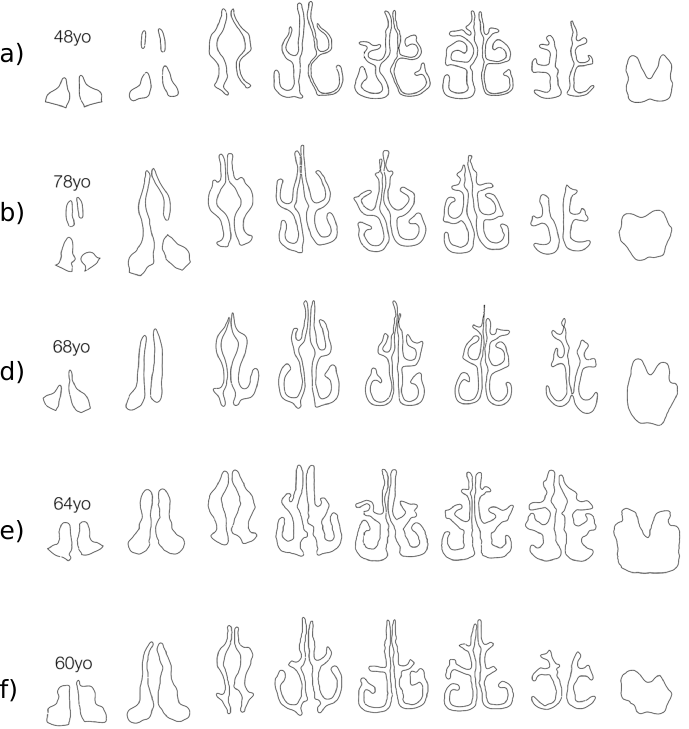
\includegraphics{Silhouettes}
  \caption{silhouettes of the cavities}
\end{figure}

\begin{figure} \label{fig:area}
  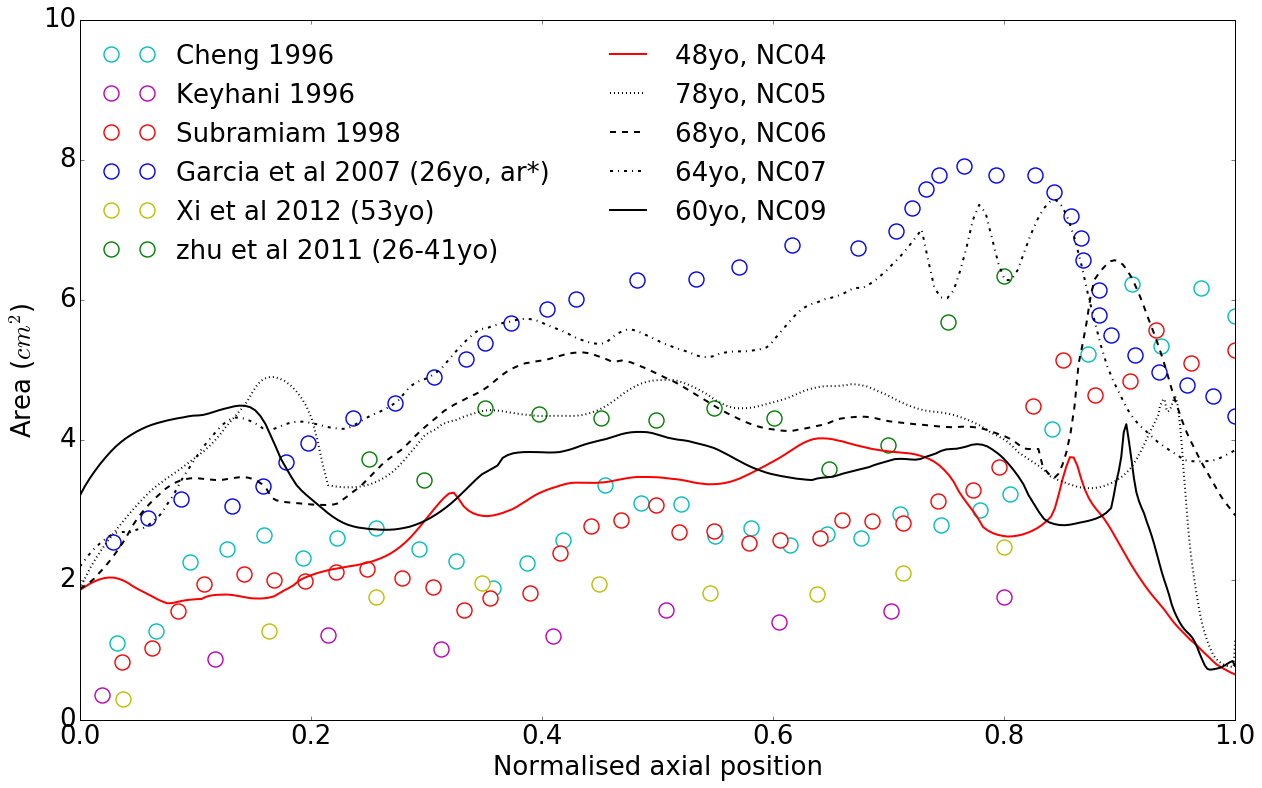
\includegraphics{Areavsdistance}
  \caption{area versus distance across the four nasal cavities with a series of examples from the literature}
\end{figure}

\begin{figure} \label{fig:arpar}
  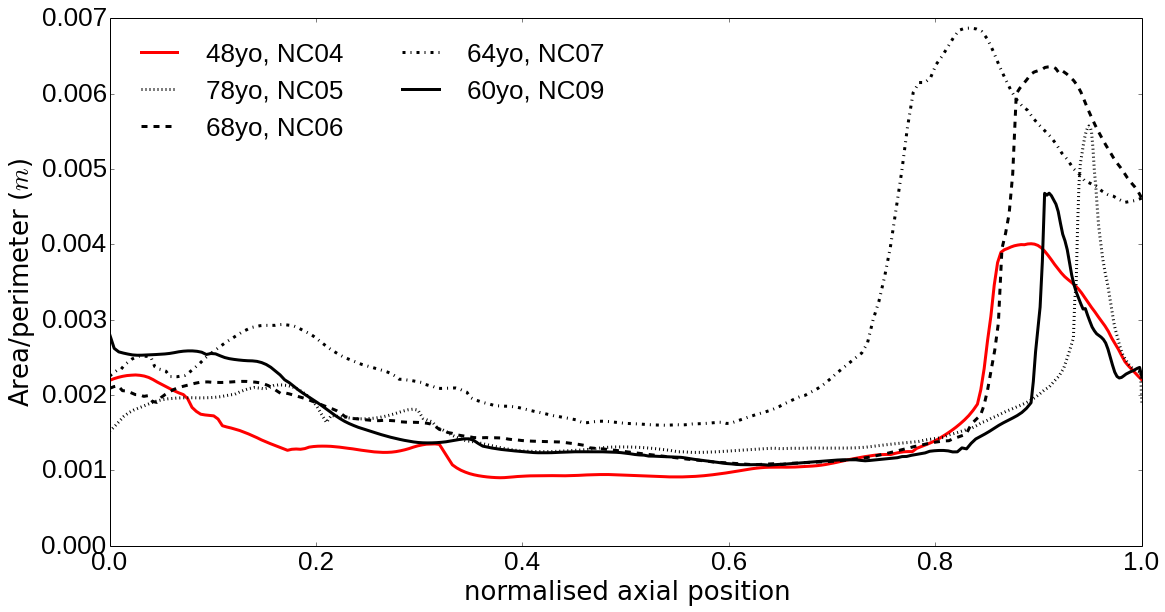
\includegraphics{areavsperimeter}
  \caption{area versus distance across the four nasal cavities with a series of examples from the literature}
\end{figure}
\section{Pressure Drop}

\begin{table}
\centering
\pgfplotstableset{
every head row/.style={before row=\toprule,after row=\midrule},
every last row/.style={after row=\bottomrule}}

\pgfplotstabletypeset[
    fixed zerofill,
    precision=2,
    display columns/0/.style={string type},
    col sep=comma]{images/prvsflow.txt}
\end{table}

\begin{figure} \label{fig:stpr}
  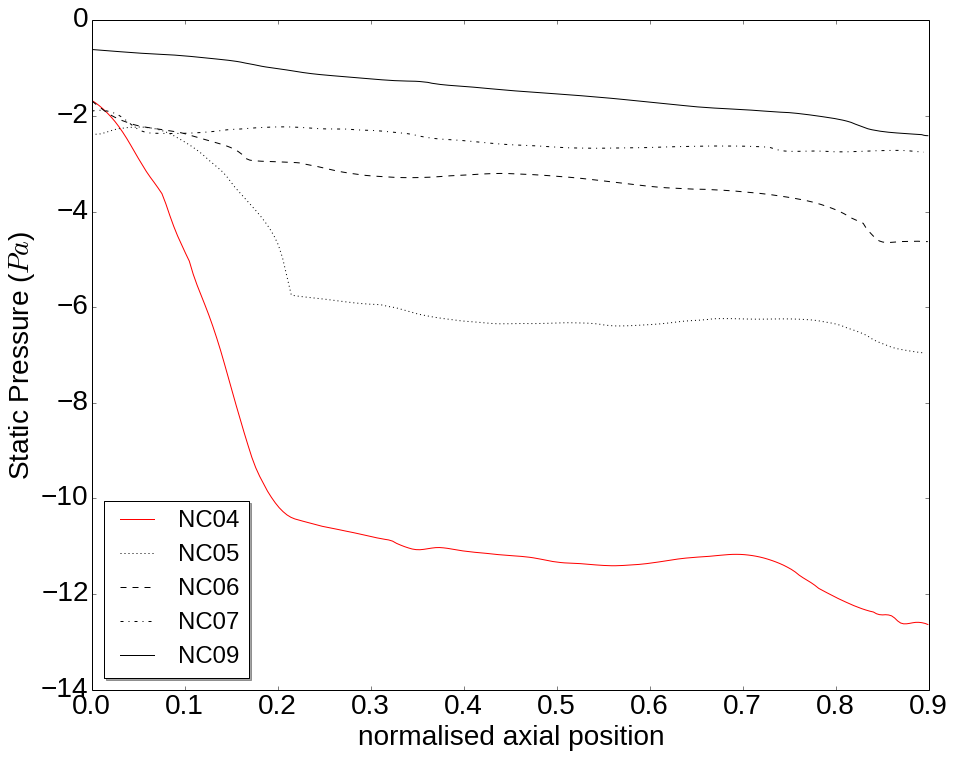
\includegraphics{statpres}
  \caption{area versus distance across the four nasal cavities with a series of examples from the literature}
\end{figure}

\section{Wall Shear Stress}

\begin{figure} \label{fig:wcont}
  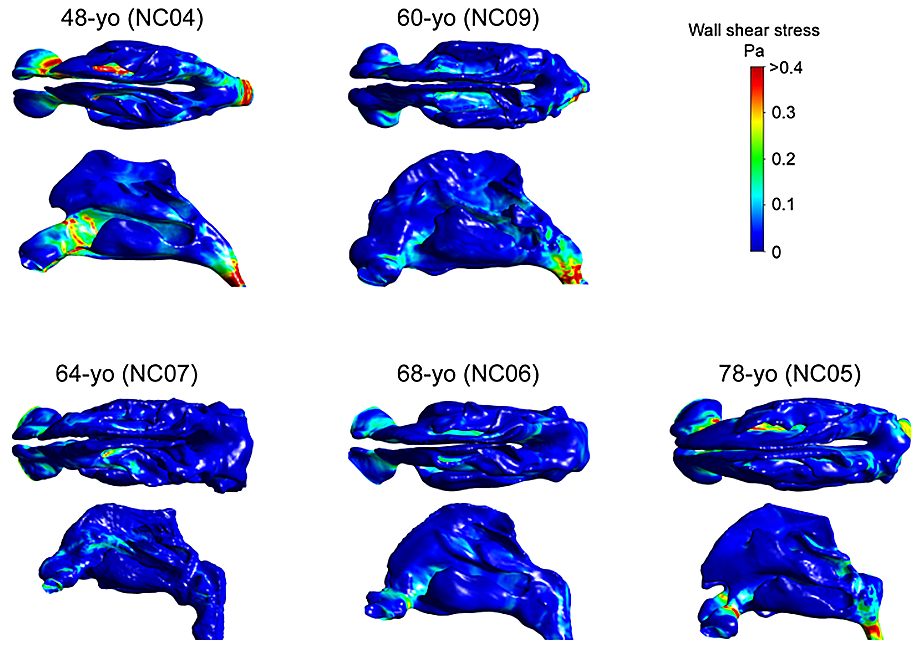
\includegraphics{wsscont}
  \caption{area versus distance across the four nasal cavities with a series of examples from the literature}
\end{figure}

\begin{figure} \label{fig:wax}
  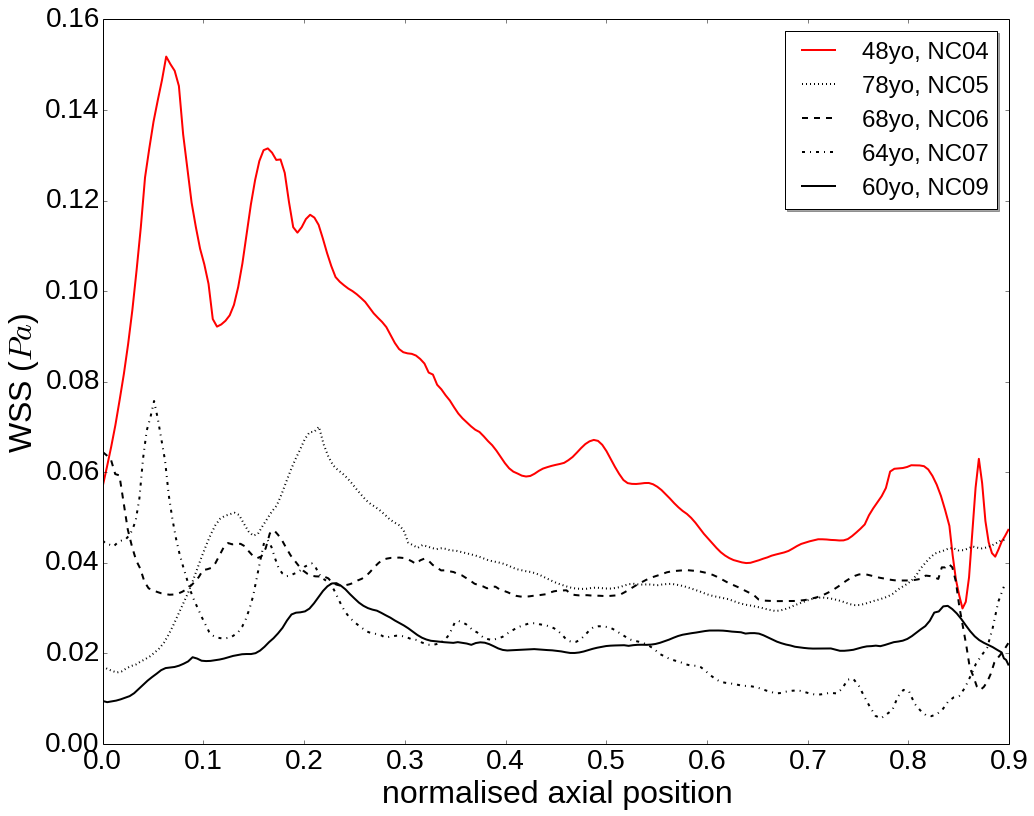
\includegraphics{axialwss}
  \caption{area versus distance across the four nasal cavities with a series of examples from the literature}
\end{figure}

\begin{figure} \label{fig:wcs}
  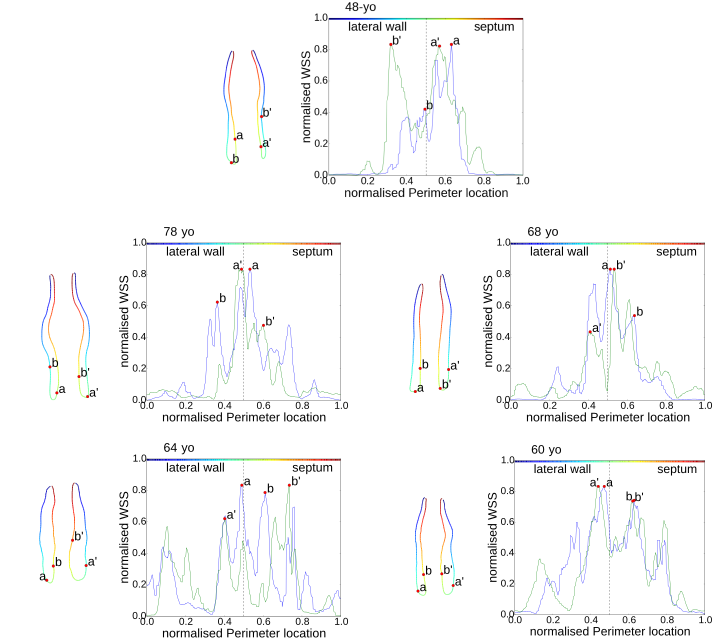
\includegraphics{wsscsvalve}
  \caption{area versus distance across the four nasal cavities with a series of examples from the literature}
\end{figure}

\begin{figure} \label{fig:wcst}
  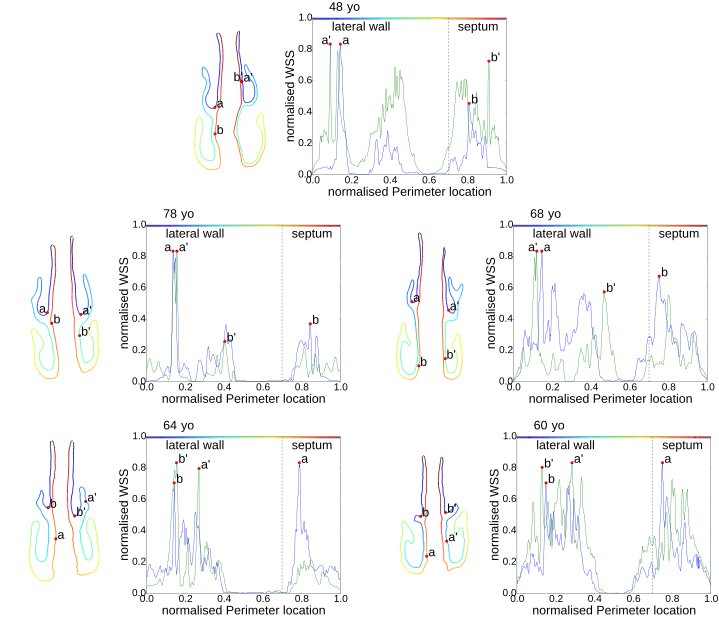
\includegraphics{wsscsturbinal}
  \caption{area versus distance across the four nasal cavities with a series of examples from the literature}
\end{figure}

\section{Velocity}


\section{Heat and Vapour Transfer}
